\section{Методы Рунге-Кутта}
Построим графики тех же зависимостей для метода Рунге-Кутта второго
(рис.~\ref{fig:rk2-errors}) и четвертого (рис.~\ref{fig:rk4-errors}) порядков,
и симплектического метода Рунге-Кутта (рис.~\ref{fig:simp-rk-errors}) что и для
метода Эйлера.
\begin{figure}[H]
    \centering
    \begin{subfigure}[b]{0.49\textwidth}
        \centering
        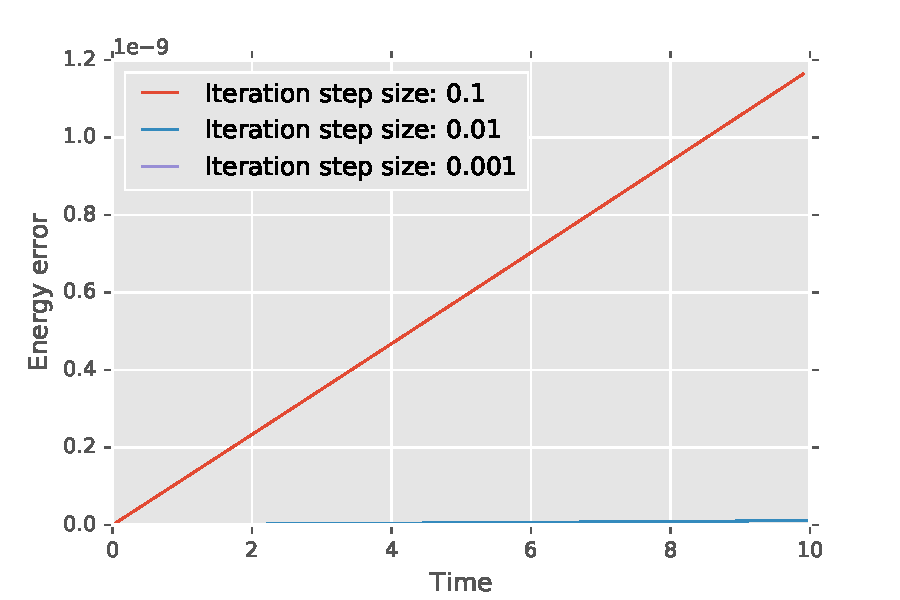
\includegraphics[width=\textwidth]{ralstonEnergy.pdf}
        \caption{}
    \end{subfigure}
    \begin{subfigure}[b]{0.49\textwidth}
        \centering
        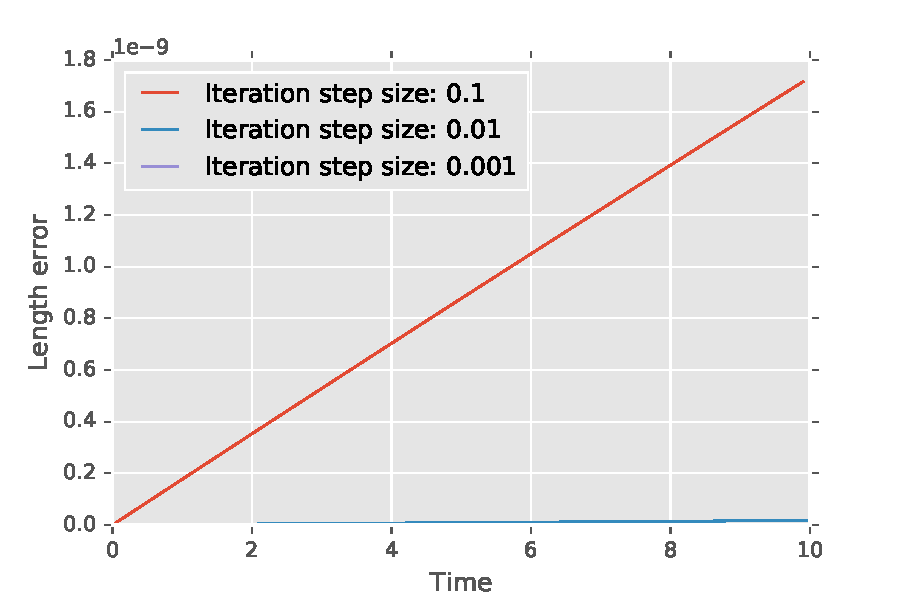
\includegraphics[width=\textwidth]{ralstonLength.pdf}
        \caption{}
    \end{subfigure}
    \caption{(а) График зависимости ошибки энергии для метода Рунге-Кутта 2го
        порядка;
        (б) График зависимости ошибки суммы длин векторов спинов для
        метода Рунге-Кутта 2го порядка.}
\label{fig:rk2-errors}
\end{figure}
\begin{figure}[H]
    \centering
    \begin{subfigure}[b]{0.49\textwidth}
        \centering
        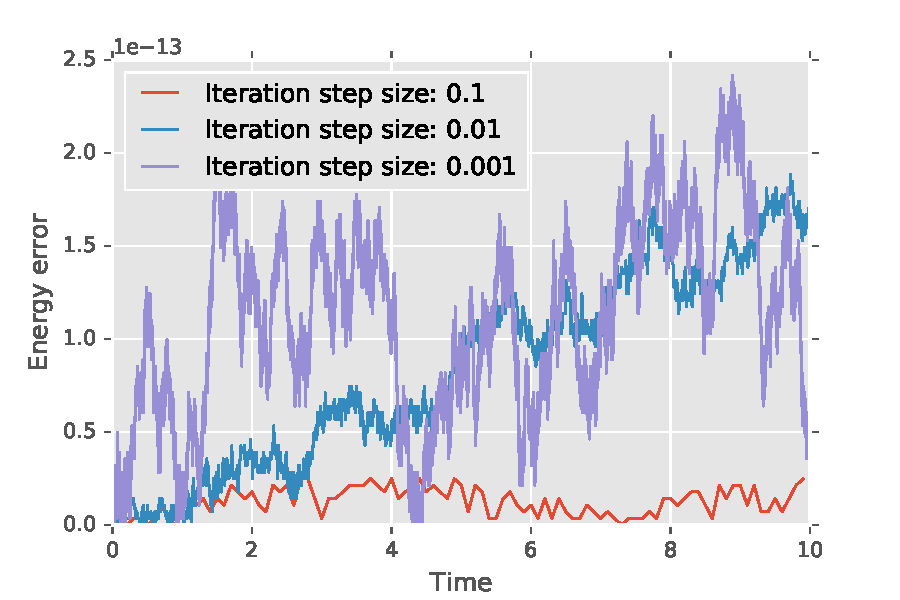
\includegraphics[width=\textwidth]{fourthEnergy.pdf}
        \caption{}
    \end{subfigure}
    \begin{subfigure}[b]{0.49\textwidth}
        \centering
        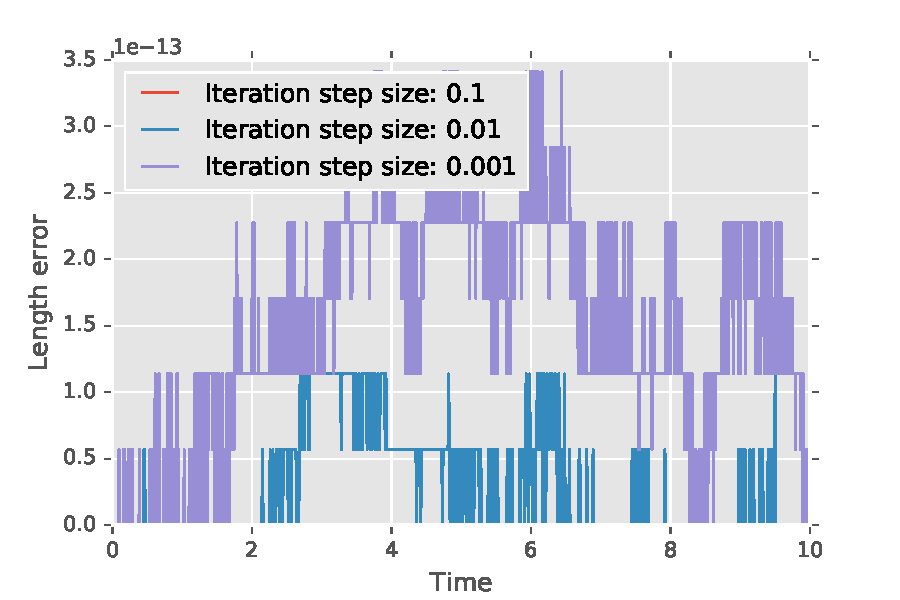
\includegraphics[width=\textwidth]{fourthLength.pdf}
        \caption{}
    \end{subfigure}
    \caption{(а) График зависимости ошибки энергии для метода Рунге-Кутта 4го
        порядка;
        (б) График зависимости ошибки суммы длин векторов спинов для
        метода Рунге-Кутта 4го порядка.}
\label{fig:rk4-errors}
\end{figure}
\begin{figure}[H]
    \centering
    \begin{subfigure}[b]{0.49\textwidth}
        \centering
        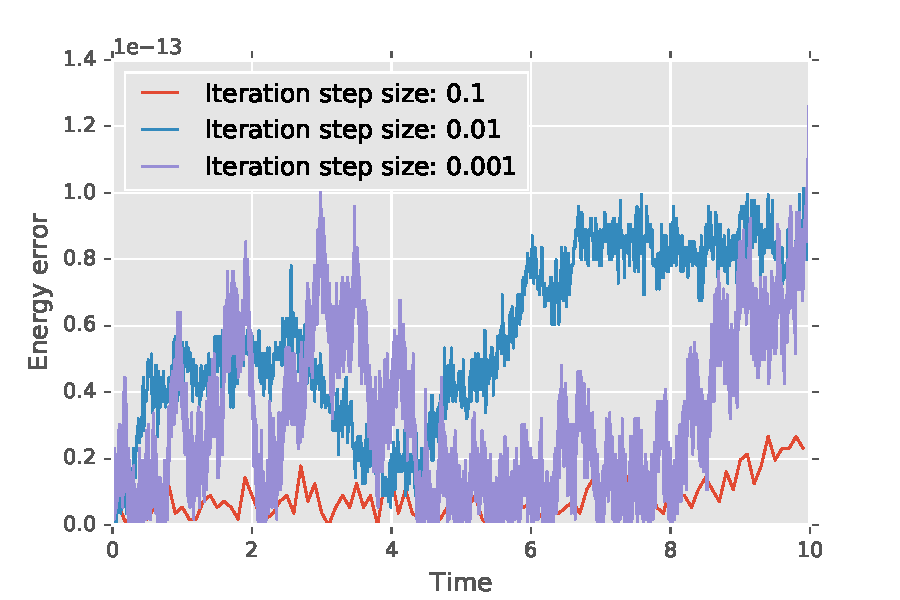
\includegraphics[width=\textwidth]{gauss2Energy.pdf}
        \caption{}
    \end{subfigure}
    \begin{subfigure}[b]{0.49\textwidth}
        \centering
        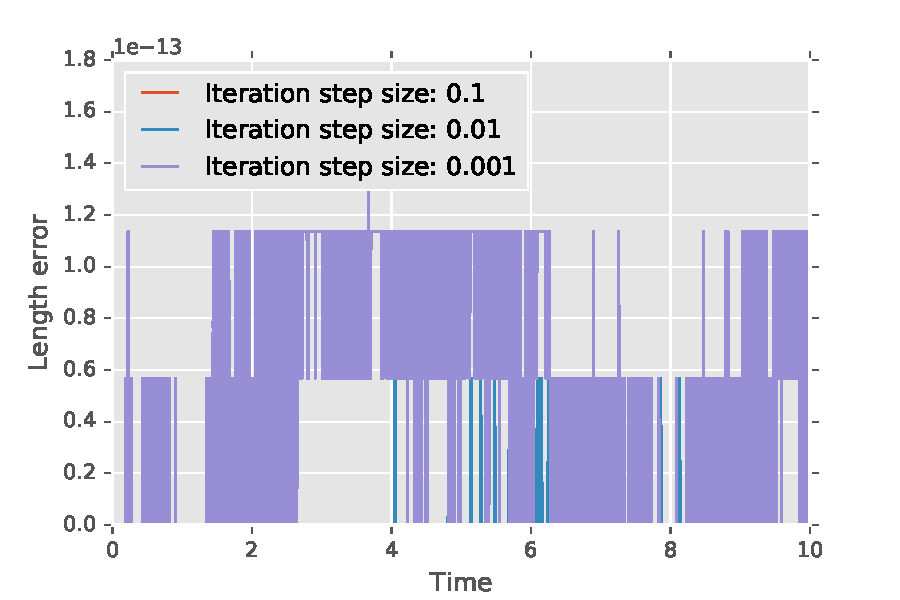
\includegraphics[width=\textwidth]{gauss2Length.pdf}
        \caption{}
    \end{subfigure}
    \caption{(а) График зависимости ошибки энергии для симплектического
        метода Рунге-Кутта;
        (б) График зависимости ошибки суммы длин векторов спинов для
        симплектического метода Рунге-Кутта.}
\label{fig:simp-rk-errors}
\end{figure}

Сравнительный график зависимости ошибки энергии, от шага интегрирования на
логарифмической шкале представленных алгоритмов, можно посмотреть на
рис.~\ref{fig:error-comparsion-energy} и ошибки суммы длин векторов на
рис.~\ref{fig:error-comparsion-length}.
\begin{figure}[H]
    \centering
    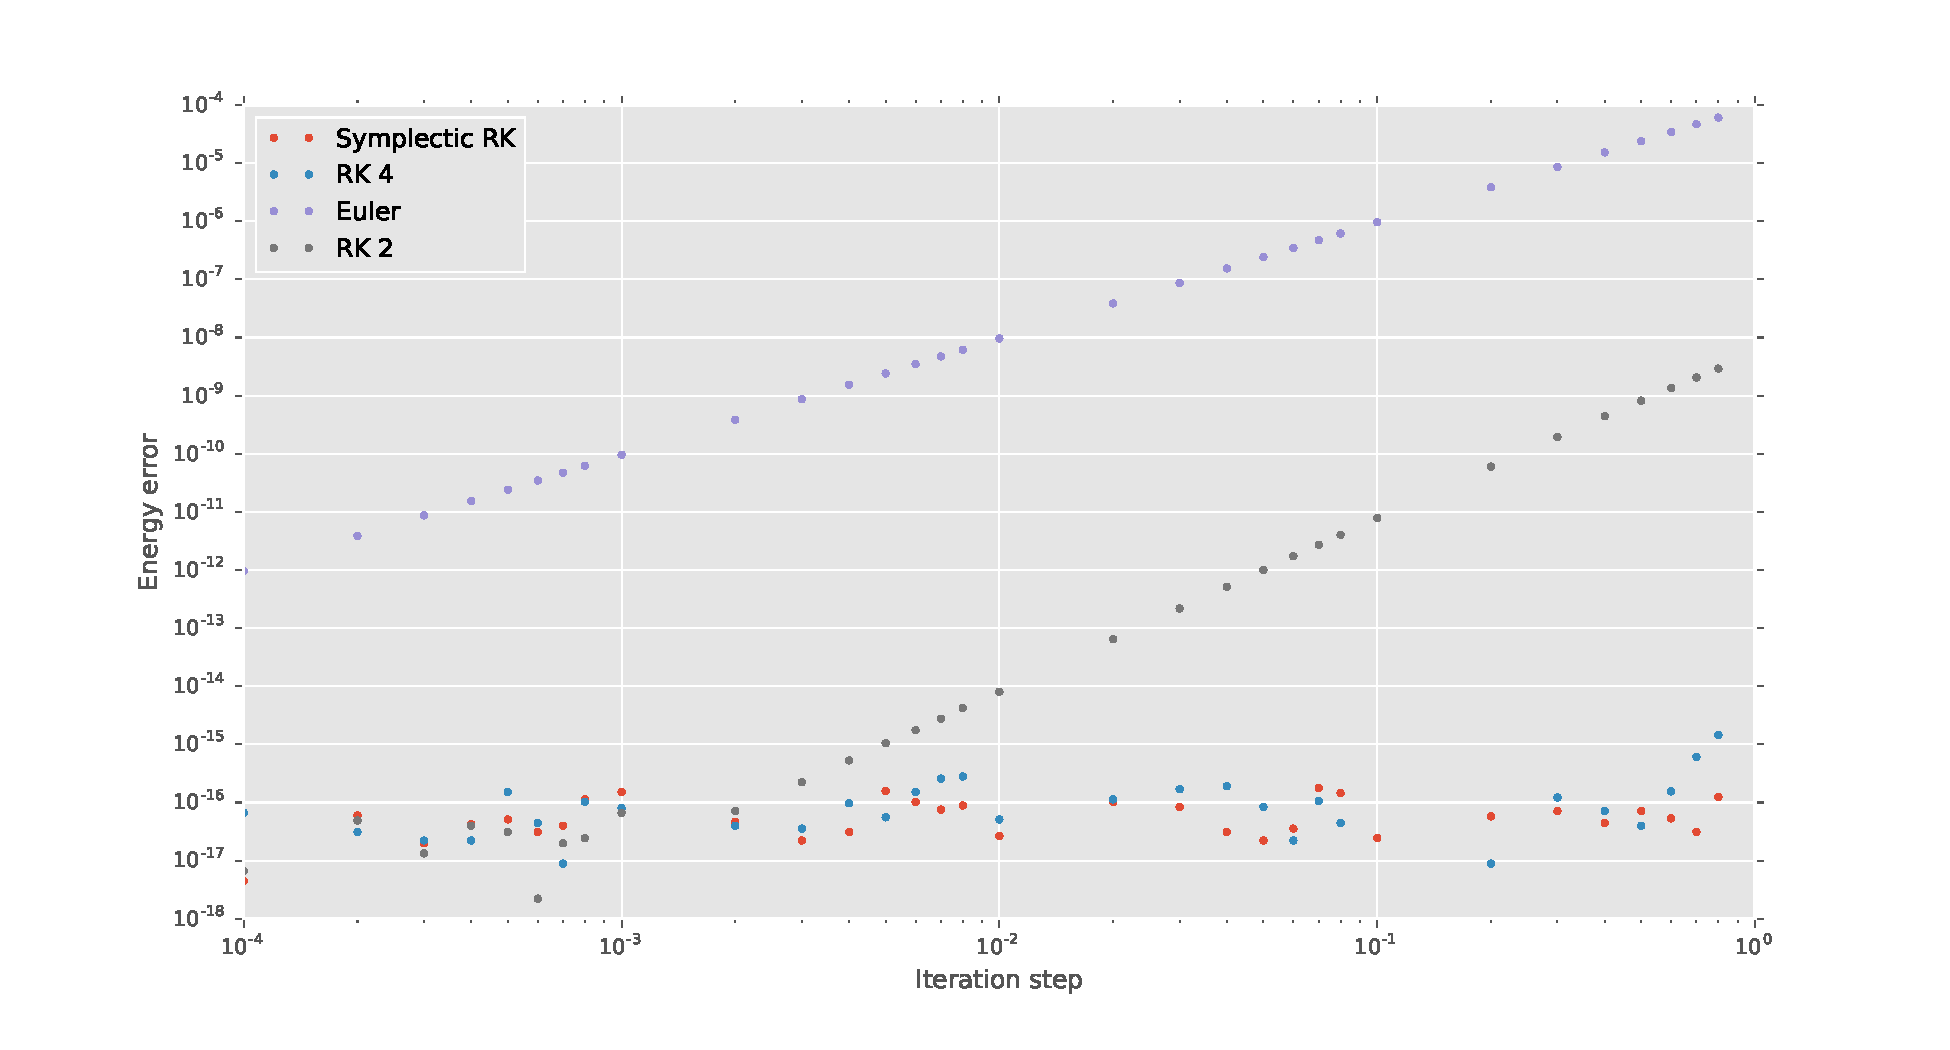
\includegraphics[width=\textwidth]{errorComparsionEnergy.pdf}
    \caption{Графики зависимости ошибки энергии от шага интегрирования на
    логарифмической шкале.}
\label{fig:error-comparsion-energy}
\end{figure}
\begin{figure}[H]
    \centering
    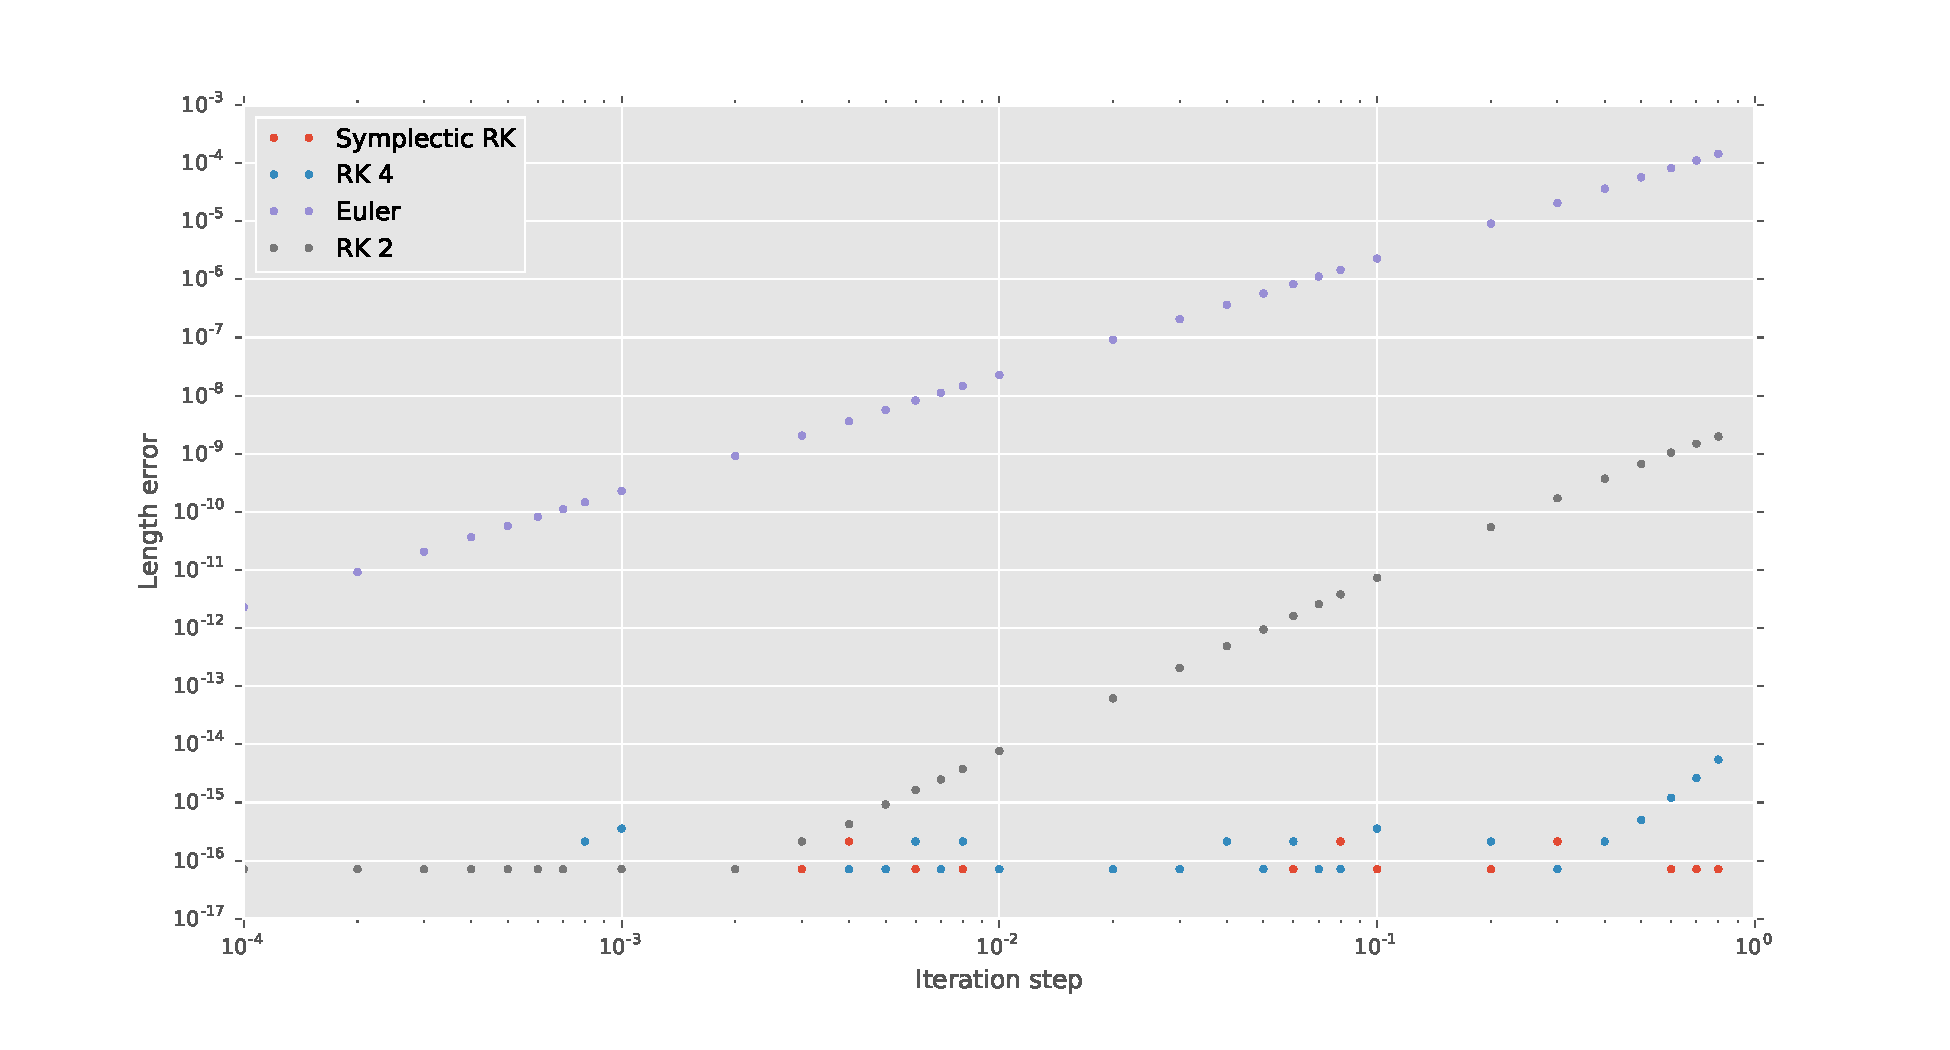
\includegraphics[width=\textwidth]{errorComparsionLength.pdf}
    \caption{Графики зависимости ошибки энергии от шага интегрирования на
    логарифмической шкале.}
\label{fig:error-comparsion-length}
\end{figure}

Сравним скорость работы алгоритмов на графиках зависимости скорости вычисления
одной итерации от размера решетки системы. Для получения следующих результатов,
алгоритмы были запущены по 1000 раз на 100 итераций с усреднением времени
выполнения одной итерации. Полученные результаты см.
рис.~\ref{fig:benchmark-speed}.
\begin{figure}[H]
    \centering
    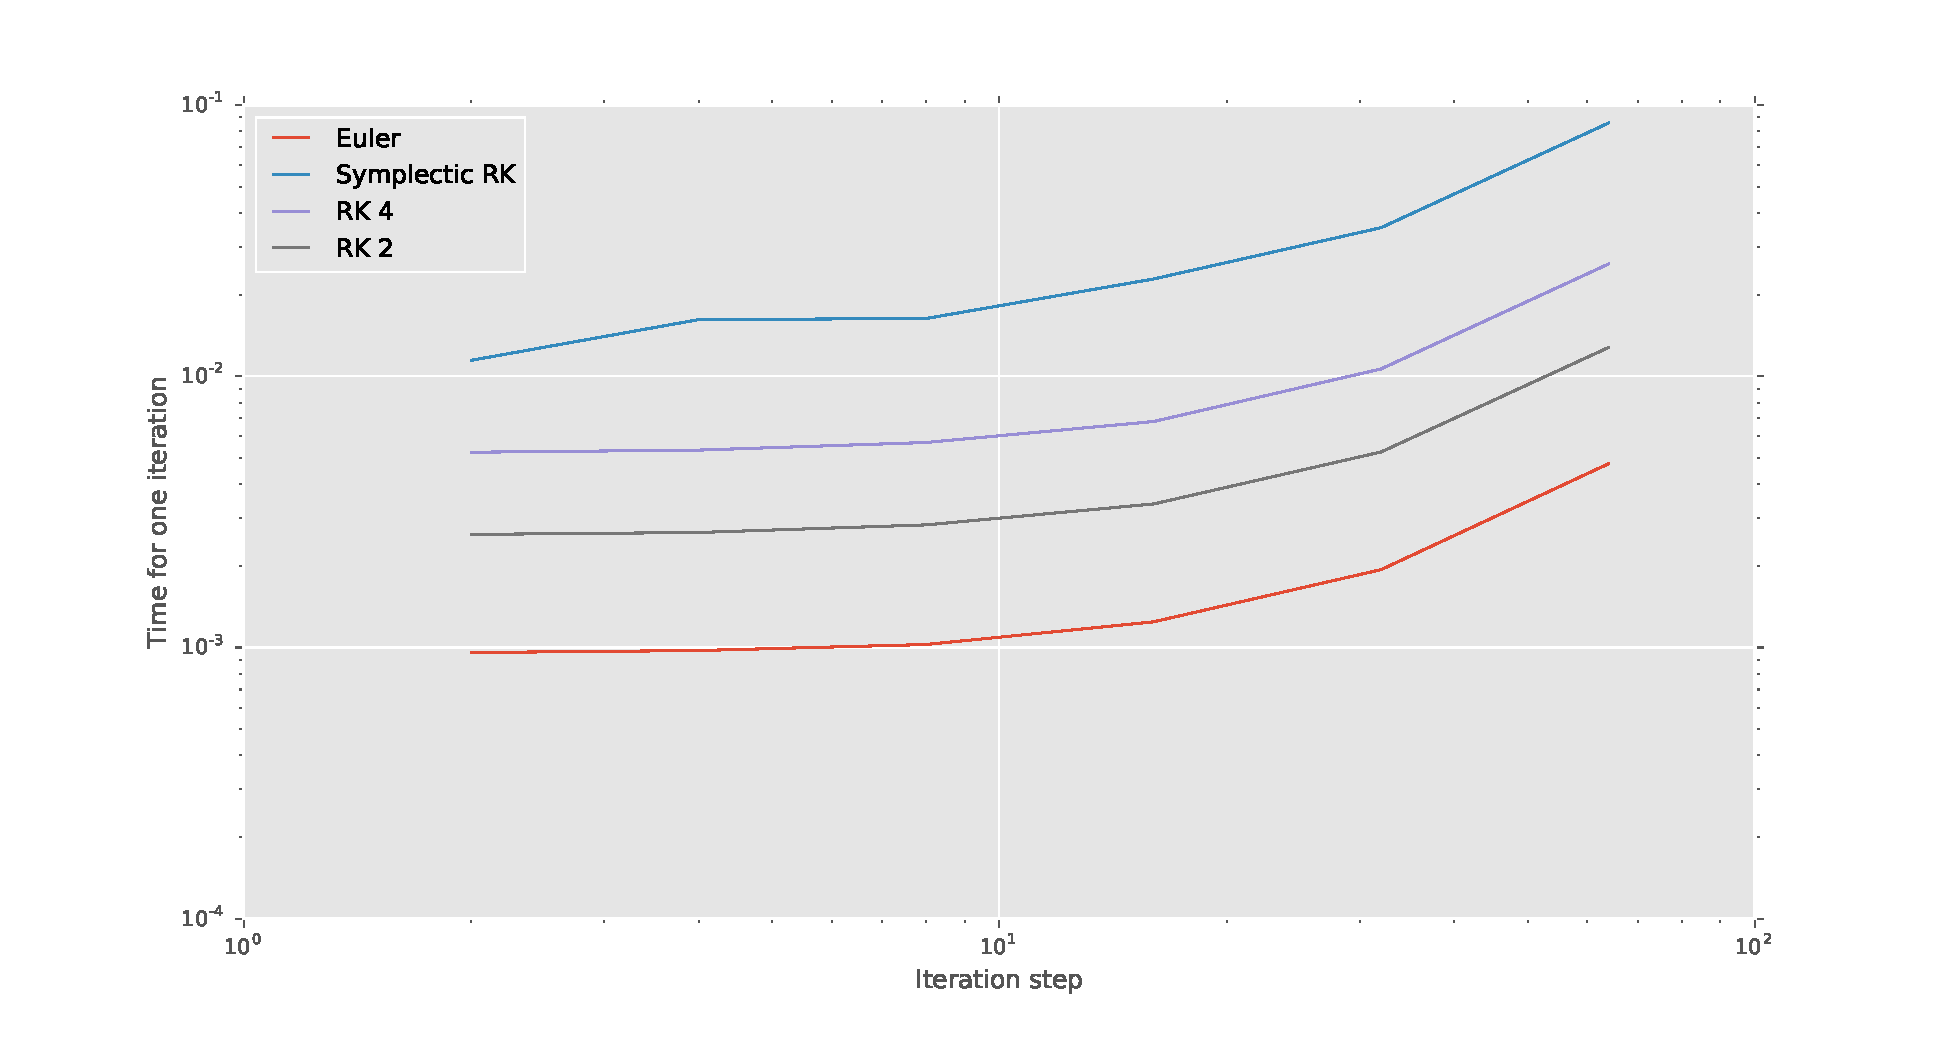
\includegraphics[width=\textwidth]{speedComparsion.pdf}
    \caption{Графики зависимости скорости вычисления одной итерации от размера
    решетки.}
\label{fig:benchmark-speed}
\end{figure}
Видно, что зависимость не линейна, на больших размерах решеток разность
скорости на одну итерацию будет не значительна, при этом предлагаемый метод
гарантирует сохранение квадратичных инвариантов на каждой итерации.

